%++++++++++++++++++++++++++++++++++++++++
% Don't modify this section unless you know what you're doing!
\documentclass[a4,11pt]{article}
\usepackage{pgfplots}
\usepackage{tabularx} % extra features for tabular environment
\usepackage{amsmath}  % improve math presentation
\usepackage{graphicx} % takes care of graphic including machinery
\usepackage[margin=1in,letterpaper]{geometry} % decreases margins
\usepackage{cite} % takes care of citations
\usepackage[final]{hyperref} % adds hyper links inside the generated pdf file
%\usepackage{gensymb}
\hypersetup{
  colorlinks=true,       % false: boxed links; true: colored links
  linkcolor=blue,        % color of internal links
  citecolor=blue,        % color of links to bibliography
  filecolor=magenta,     % color of file links
  urlcolor=blue         
}
\usepackage{float}
\makeatletter
\newcommand*{\rom}[1]{\expandafter\@slowromancap\romannumeral #1@}
\makeatother
%++++++++++++++++++++++++++++++++++++++++


\begin{document}
\title{NTC Thermistor Sensor}
\author{Catherine Beryl Basson, Piotr Chromi\'nski}
\date{13 December 2016}
\maketitle
\twocolumn
\section{Introduction}

The NTC thermistors display non-linear resistance characteristics with temperature. The resistance of an NTC will decrease at the temperature increases. This behaviour is related to it's constant value $B$. This phenomenon allows for use of an NTC thermistor as a temperature sensor. In the discussed experiments a Vishay NTCLE100E3 thermistor was used, with $B=3977^{\circ}K$.

\section{Experiments}
Two experiments were conducted. First, to determine characteristics of the non-linear response of the NTC: resistance-temperature R-T and temperature-resistance T-R, maximum non-linearity $\hat N$ as \% of full scale deflection $f.s.d$; response of a system linearised by a parallel resistor. Second, to find the time constant $\tau$ of the measurement system. Raw data of all measurements is presented in the Apendix.
\subsection{R-T Characteristics}

To measure the R-T and T-R characteristics the resistance was measured with an AMPROBE AM-510-EUR multimeter, and recorded over temperature range 90--45$^{\circ}C$. This was achieved by measuring the temperature of water in a cup, which was cooled from$~100^{\circ}$ to$~45^{\circ}$.

To determine the parallel resistor value $R_{T_{ctr}}$ was recorded at $T_{ctr}=72.5^{\circ}C$ and calculated using the eqation.
\subsection{Time Constant}
\section{Results}
\subsection{R-T Characteristics}
\subsection{Time Constant}
\subsubsection{Non-Linear}

Equation for expected intermediate temperatures, taken from the thermistor's datasheet here modified for temperature $T$ in $^{\circ}C$
$$R_{(T)}=R_{ref}\cdot e^{A+\frac{B}{T+273.15}+\frac{C}{(T+273.15)^2}+\frac{D}{(T+273.15)^3}}$$
Where $A$, $B$, $C$, and $D$ are constant values which are dependent on the thermistor; $R_{ref}$ is the resistance at a reference temperature---for the thermistor used in the experiment it is $10000\Omega$.

\begin{figure}[H]
  \centering
  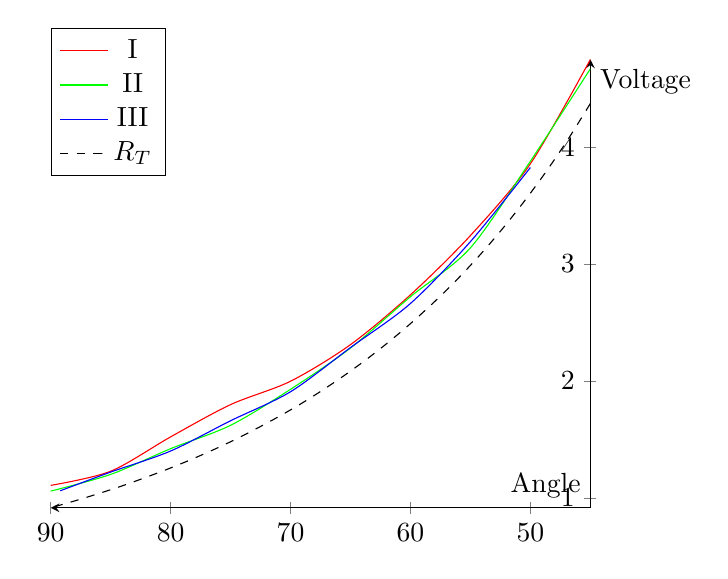
\begin{tikzpicture}
    \begin{axis}[
      axis lines=middle,
      x dir=reverse,
      legend style={
        at={(axis cs:90,3.75)},
        anchor=south west},
      xlabel=Angle, ylabel=Voltage]
      \addplot[smooth,
      color=red,
      mark=none,
      error bars/.cd,y dir=both,
      y explicit] coordinates {
        (90, 1.107)
        (85, 1.228)
        (80, 1.522)
        (75, 1.798)
        (70, 1.998)
        (65, 2.311)
        (60, 2.737)
        (55, 3.244)
        (50, 3.858)
        (45, 4.75)
      };
      \addlegendentry{\rom{1}}
      \addplot[smooth,
      color=green,
      mark=none,
      error bars/.cd,y dir=both,
      y explicit] coordinates {
        (90, 1.058)
        (85, 1.201)
        (80, 1.421)
        (75, 1.621)
        (70, 1.929)
        (65, 2.282)
        (60, 2.721)
        (55, 3.139)
        (50, 3.88)
        (45, 4.67)
      };
      \addlegendentry{\rom{2}}
      \addplot[smooth,
      color=blue,
      mark=none,
      error bars/.cd,y dir=both,
      y explicit] coordinates {
        (89.2, 1.061)
        (85, 1.221)
        (80, 1.401)
        (75, 1.66)
        (70, 1.908)
        (65, 2.286)
        (60, 2.663)
        (55, 3.192)
        (50, 3.826)
      };
      \addlegendentry{\rom{3}}
      \addplot[smooth, black, dashed][domain=45:90]{10*exp(-14.6337+(4791.842/(x+273.15)+(-115334/((273.15 + x)^2))+((-3.730535*1000000)/((273.15 + x)^3)))};
      \addlegendentry{$R_T$}
    \end{axis}
  \end{tikzpicture}
  \label{fig:actual}
  without parallel resistor
\end{figure}
\subsubsection{Linear}
\section{Error Discussion}
\section{Tables}
\section{Equations}

Equation for parallel linearising resistor taken from Siemens Note(?):
$$R_p=R_{T_{ctr}}\cdot\frac{B-T_{ctr}}{B+2T_{ctr}}$$
where $R_{T_{ctr}}$ is thermistor resistance at the center temperature $T_{ctr}$ and $B$ is the $B$ value of a thermistor.
\section{Graphs}
\begin{figure}[h]
  \centering
  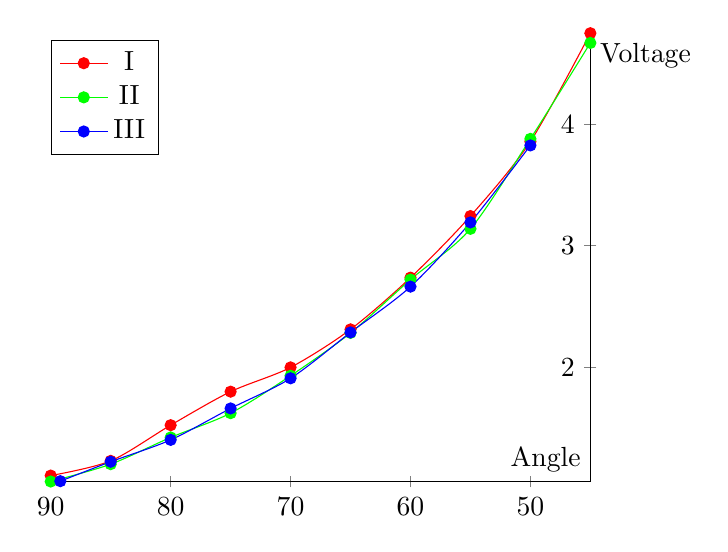
\begin{tikzpicture}
    \begin{axis}[
      axis lines=middle,
      x dir=reverse,
      legend style={
        at={(axis cs:90,3.75)},
        anchor=south west},
      xlabel=Angle, ylabel=Voltage]
      \addplot[smooth,
      color=red,
      mark=*,
      error bars/.cd,y dir=both,
      y explicit] coordinates {
        (90, 1.107)
        (85, 1.228)
        (80, 1.522)
        (75, 1.798)
        (70, 1.998)
        (65, 2.311)
        (60, 2.737)
        (55, 3.244)
        (50, 3.858)
        (45, 4.75)
      };
      \addlegendentry{\rom{1}}
      \addplot[smooth,
      color=green,
      mark=*,
      error bars/.cd,y dir=both,
      y explicit] coordinates {
        (90, 1.058)
        (85, 1.201)
        (80, 1.421)
        (75, 1.621)
        (70, 1.929)
        (65, 2.282)
        (60, 2.721)
        (55, 3.139)
        (50, 3.88)
        (45, 4.67)
      };
      \addlegendentry{\rom{2}}
      \addplot[smooth,
      color=blue,
      mark=*,
      ] coordinates {
        (89.2, 1.061)
        (85, 1.221)
        (80, 1.401)
        (75, 1.66)
        (70, 1.908)
        (65, 2.286)
        (60, 2.663)
        (55, 3.192)
        (50, 3.826)
      };
      \addlegendentry{\rom{3}}
    \end{axis}
  \end{tikzpicture}
  \label{fig:actual}
  without parallel resistor
\end{figure}

\begin{figure}[h]
  \centering
  \begin{tikzpicture}
    \begin{axis}[
      axis lines=middle,
      x dir=reverse,
      ]
      \addplot[smooth, black, dashed][domain=25:90]{10000*exp(-14.6337+(4791.842/(x+273.15)+(-115334/((273.15)^2))+((-3.730535*1000000)/((273.15)^3)))};
    \end{axis}
  \end{tikzpicture}
  \label{fig:actual}
  $$R_{(T)}=R_{ref}\cdot e^{A+\frac{B}{T}+\frac{C}{T^2}+\frac{D}{T^3}}$$
  with parallel resistor
\end{figure}

\section{Conclusion}
\end{document}
